\documentclass[]{amsart}
\setlength{\marginparwidth}{0.5in}
\usepackage{amsmath,amssymb,amsthm,mathtools,booktabs,array,tikz,pifont,comment,graphicx}
\usepackage[author-year]{amsrefs}
\input FJHDef.tex

%Requires ApproxUnivariate.tex, univariate_integration.tex, foolbwquadexample.eps 

\DeclareMathOperator{\Var}{Var}
\DeclareMathOperator{\INT}{INT}
\DeclareMathOperator{\lin}{lin}
\DeclareMathOperator{\up}{up}
\DeclareMathOperator{\lo}{lo}
\DeclareMathOperator{\fix}{non}
\DeclareMathOperator{\err}{err}
\DeclareMathOperator{\maxcost}{maxcost}
\DeclareMathOperator{\mincost}{mincost}
\newcommand{\herr}{\widehat{\err}}

\newtheorem{theorem}{Theorem}
\newtheorem{prop}[theorem]{Proposition}
\newtheorem{lem}{Lemma}
\newtheorem{cor}{Corollary}
\theoremstyle{definition}
\newtheorem{algo}{Algorithm}
\newtheorem{condit}{Condition}
%\newtheorem{assump}{Assumption}
\theoremstyle{remark}
\newtheorem{rem}{Remark}
\newcommand{\Fnorm}[1]{\abs{#1}_{\cf}}
\newcommand{\Gnorm}[1]{\abs{#1}_{\cg}}
\newcommand{\flin}{f_{\text{\rm{lin}}}}


\begin{document}

\title{Reliable Automatic Quadrature for Cones of Integrands}
\author{Fred J. Hickernell}
\author{Martha Razo}
\author{Sunny Yun}
\maketitle 


\begin{abstract} Hi
\end{abstract}


\section{Introduction} 

Automatic numerical algorithms for univariate integration appear in many widely used software packages, such as MATLAB \ycite{MAT8.1}, Mathematica \ycite{Mat9a}, NAG \ycite{NAG23}, and R \ycite{R2512}.  Automatic algorithms determine adaptively where and how much to sample the integrand by estimating the algorithm error from the sampled function values.  Unfortunately, such error estimation methods are unreliable, as pointed out by James Lyness \ycite{Lyn83}.

Here we show how to overcome Lyness's objections by employing a new paradigm for error bounds, which is based on cones, rather than balls, of integrands rather than balls.  This article illustrates with greater detail the more general setting in \ocite{HicEtal14b}.  We argue that the traditional way of teaching error estimation for numerical integration should be changed to reflect this new paradigm.  Moreover, this paradigm can, and should, be applied to other problems requiring automatic algorithms. 

\subsection{Why Numerical Integration Is Needed?}
Soon after a calculus student first learns about integration, she learns that the integrals of many elementary functions are \emph{not} themselves elementary functions.  An important example is the standard normal probability density function, $\phi: x \mapsto \me^{-x^2}/\sqrt{2 \pi}$.  Since the antiderivative of $\phi$ cannot be expressed in terms of elementary functions, values of the standard normal distribution function $\Phi : x \mapsto \int_{-\infty}^x \phi(t) \, \dif t$ must be provided in tables in textbooks and special functions in calculators. By contrast, the derivatives of elementary functions are elementary functions.  

\subsection{The Trapezoidal Rule}
Students need to know that no analytic answer does not mean no answer, so calculus students are often introduced to numerical integration (quadrature) methods such as the trapezoidal rule, $T_n$:
\begin{equation}
\int_0^1 f(x) \, \dif x \approx T_n(f) := \frac{1}{2n} \left [ f(0) + 2 f(1/n) + \cdots + 2 f(1-1/n) + f(1) \right].
\end{equation}
One may ask ``How large should the number of trapezoids, $n$, be so that the absolute error of $T_n(f)$ does not exceed a tolerance $\varepsilon$?''  Theoretical and rigorous error bounds are proportional to $1/n^2$, e.g., \ocite{BraPet11a}*{Sect.\ 7.2, (7.15)}: 
\begin{equation} \label{traperrbd}
\err(f,n) := \abs{\int_0^1 f(x) \, \dif x - T_n(f)} \le \frac{\Var(f')}{8n^2}, \qquad n \in \naturals = \{1, 2, \ldots \}. 
\end{equation}
The error bound is also proportional to the total variation of the first derivative of the integrand.  The total variation, $\Var(\cdot)$, is defined as
\begin{equation} \label{vardef}
\Var(f) := \sup_{\substack{n \in \naturals\\ 0 = x_0 < x_1 < \cdots < x_{n} =1}} \sum_{i=1}^n \abs{f(x_i)-f(x_{i-1})}.
\end{equation}
The trapezoidal rule approximates the integrand by a piecewise linear spline and thus gives the exact answer for such integrands.  Error bound \eqref{traperrbd} reflects this since  $\Var(f')$ vanishes when $f(x)=ax+b$.

The total variation is closely related to the $\cl_1$-norm:
\begin{gather*}
\Var(f)= \norm[1]{f'} \text{ if } \norm[1]{f'}< \infty, \\ 
\text{where} \qquad \qquad \norm[p]{f}:= \begin{cases} \displaystyle \left[\int_0^1 \abs{f(x)}^p \, \dif x \right]^{1/p}, & 1 \le p < \infty,\\[1ex]
\displaystyle  \sup_{0 \le x \le 1} \abs{f'(x)}, & p=\infty.
\end{cases}
\end{gather*}
Error bounds resembling \eqref{traperrbd} exist in terms of $\norm[p]{f''}$ for $1 \le p \le \infty$ with leading constants depending on $p$.  

If $f$ has a simple form, one might be able to derive an upper bound on $\Var(f')$ and turn error bound \eqref{traperrbd} into an automatic algorithm.  The algorithm below is guaranteed to produce $\err(f,n)\le \varepsilon$ provided that $\Var(f') \le M_1$.  

\begin{algo} Given an error tolerance, $\varepsilon$, set 
\begin{equation}\label{algo1n}
n = \left \lceil \sqrt{M_1/(8\varepsilon)} \right \rceil,
\end{equation}
and return the trapezoidal rule approximation $T_n(f)$ as the answer.
\end{algo}

For example, for $\phi$ defined above, $\Var(f')=1/\sqrt{2 \pi \me}$, and so one may choose any $n \ge 1/\sqrt{8\sqrt{2 \pi \me} \, \varepsilon}$.  However, not all integrands have first derivatives whose variations are so easy to bound.  

\section{The Flaws in the Prevalent Data-Based Error Estimate}
Automatic quadrature algorithms do not require the user to specify $M_1$, but bound or estimate the error based solely on the function values, $f(x_i)$, and then determine the sample size accordingly.  Here we focus on this error estimation process.  As we demonstrate in this section, the popular error estimate for the trapezoidal rule is flawed. 

Numerical methods texts, such as \ocite{BurFai10}*{p.\ 223--224}, \ocite{CheKin12a}*{p.\ 233}, and  \ocite{Sau12a}*{p.\ 270}, advise readers to estimate the error of $T_n(f)$ in terms of its from $T_{n/2}(f)$, specifically,
\begin{equation}\label{baderr}
\herr(f,n) = \frac{\abs{T_n(f) - T_{n/2}(f)}}{3}, \qquad \frac n2 \in \naturals.
\end{equation}
This algorithm leads to the following automatic and adaptive quadrature algorithm.

\begin{algo} \label{baderralgo} Given an error tolerance, $\varepsilon$, let $j=1$ and $n_1=2$.

\begin{description} 

\item[Stage 1] Compute the error estimate $\herr(f,n_j)$ according to \eqref{baderr}.

\item [Stage 2] If $\herr(f,n_j) \le \varepsilon$, then return the trapezoidal rule approximation $T_{n_j}(f)$ as the answer.  

\item [Stage 3] Otherwise let $n_{j+1}=2 n_j$, increase $j$ by one, and go to Stage 1.

\end{description}

\end{algo}

By doubling the number of trapezoids for each iteration, the data from the previous iterations can be reused.  Automatic quadrature algorithms in commonly used numerical libraries are more sophisticated than Algorithm \ref{baderralgo}, but their stopping criteria are similar in spirit and have the same intrinsic flaws.

While, Algorithm \ref{baderralgo} requires no a priori bound on the variation of the first derivative of the integrand, there is no guarantee that $\err(f,n)\le \varepsilon$.  In fact, one may easily to construct integrands, $f$, such that this error estimate fails completely, e.g.,
\begin{equation} \label{failcond}
\int_0^1 f(x) \, \dif x =  1, \quad T_{n}(f)=T_{n/2}(f) = -1, \quad \err(f,n)=2 \ne 0 = \herr(f,n).
\end{equation}
Figure \ref{spikeflukefig} shows  examples of two integrands satisfying these conditions. These two integrands illustrate two ways in which the error estimate $\herr(\cdot)$, and Algorithm \ref{baderralgo}, can fail.  One way is ultimately unavoidable but ought to be quantifiable.  The other way is inexcusable, but is prevalent in widely used automatic numerical quadrature.

\begin{figure}
\centering 
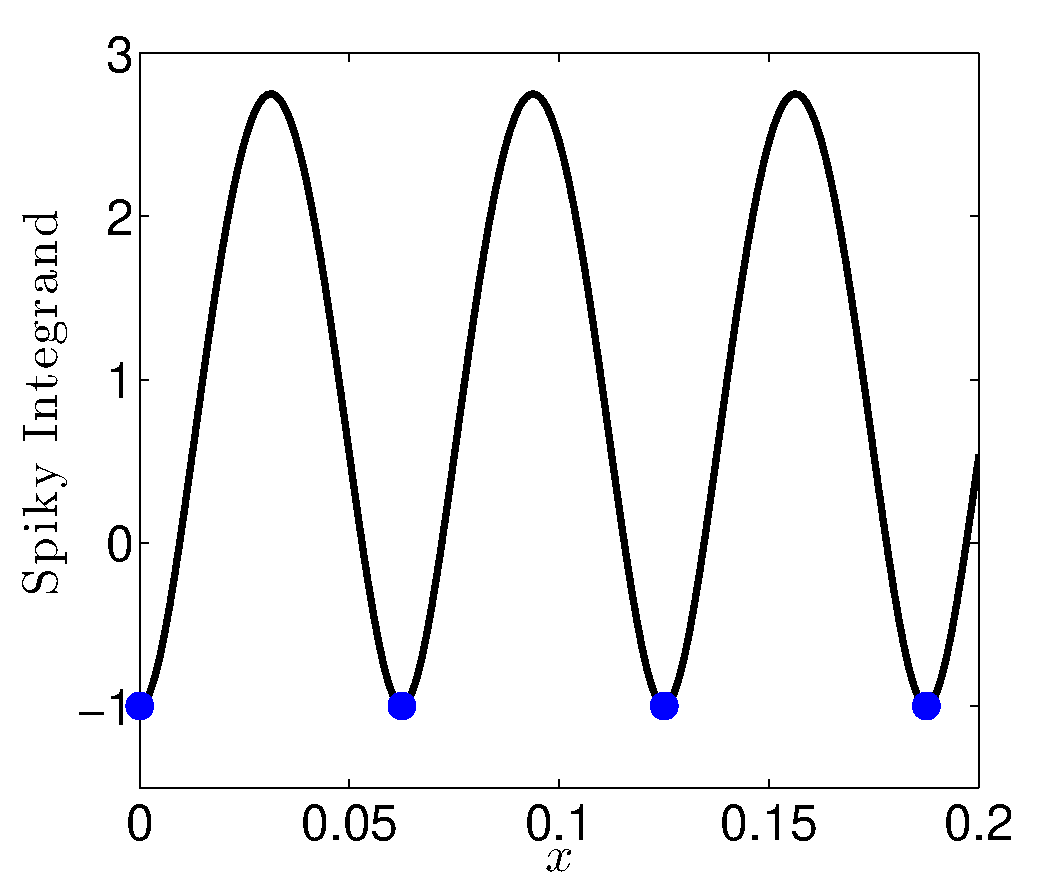
\includegraphics[width=6cm]{SpikyIntegFigcolor.eps} \quad
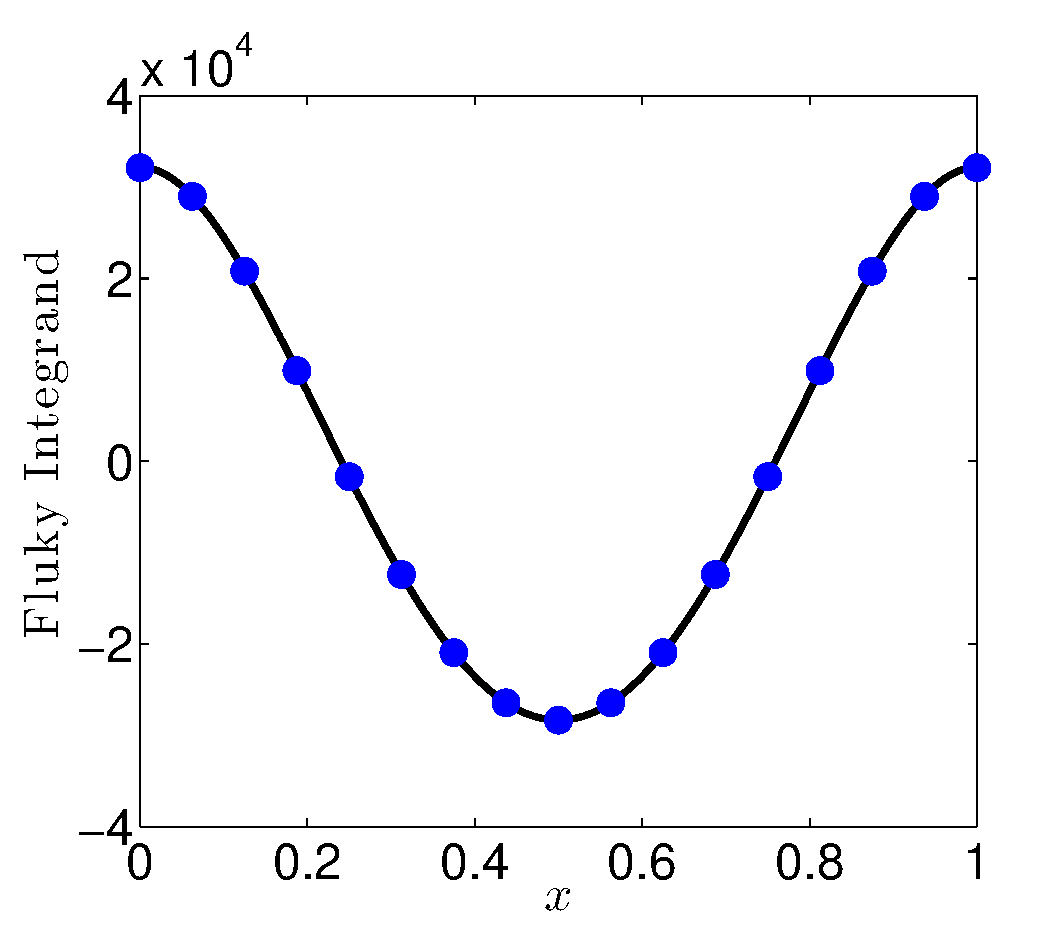
\includegraphics[width=6cm]{FlukyIntegFigcolor.eps}
\caption{Examples of a spiky integrand (left) and a fluky integrand (right), which satisfy the failure conditions \eqref{failcond} for $n=32$. \label{spikeflukefig}}
\end{figure}

\subsection{Spiky Integrands} \emph{Any} quadrature algorithm that depends only on function values to estimate error will be fooled by sufficiently spiky integrands.  Suppose that the quadrature algorithm samples the integrand at a seqeunce of points, $\xi_1, \xi_2, \ldots$, and suppose that $f(\xi_i)$ is the same value for all $\xi_i$.  Here the algorithm may even be adaptive, meaning that $\xi_{i+1}$ may depend on $(\xi_1, f(\xi_1)), \ldots, (\xi_i, f(\xi_i))$.  Eventually the algorithm stops at $n$ points.  Under mild conditions on the set of integrands of interest the best estimate of the integral is that constant. 

Figure \ref{spikeflukefig} (left) plots the following spiky integrand that is defined in terms of the quartic Bernoulli polynomial:
\begin{equation} \label{spiky}
f_{\text{spiky}}(x;n) = 1 + 60 B_4(\bbl nx \bbr), \qquad n \in \naturals, \quad \bbl x \bbr := x \bmod 1.
\end{equation}
The Bernoulli polynomials are described by \ocite{AbrSte64}*{Chap.\ 23, \url{http://dlmf.nist.gov/24}}.  The first six are defined as follows 
\begin{subequations} \label{Bernoulli}
\begin{gather} 
B_0(x) = 1, \qquad B_1(x) = x-1/2,  \qquad 
B_2(x)=1/6 - x(1-x), \\ 
B_3(x) = \frac{1}{2} x(1-x)(1-2x), \qquad B_4(x) = -1/30 + [x(1-x)]^2, \\
B_5(x) = \frac{1}{6} x(1-x)(1-2x)(1 + 3 x - 3 x^2).
\end{gather}
\end{subequations}
The integrand $f_{\text{spiky}}(\cdot;n)$ satisfies \eqref{failcond} for even $n$ and has 
\begin{itemize}
\item $n+1$ local minima of $-1$ at $x=0, 1/n, \ldots, 1$, and
\item $n$ local maxima of $11/4$ at $x=1/(2n), 3/(2n), \ldots, 1-1/(2n)$.
\end{itemize}

The problem of integrating spiky functions never goes away, but it should be quantifiable.  An algorithm ought to integrate functions accurately, provided that they have spikes no thinner than say, $\delta$.  Moreover, the algorithm should be tunable so that the user can specifiy $\delta$.  We describe such an algorithm in Section \ref{newalgosec}, along with a precise definition of spike width.

\subsection{Fluky Integrands} 

Thirty years ago James Lyness wrote a SIAM Review article, \emph{When Not to Use an Automatic Quadrature Routine}.  While recognizing the problem of spiky integrands, he claims that there is even a more serious problem with automatic quadrature methods   \cite{Lyn83}*{p.\ 69}:
\begin{quote}
While prepared to take the risk of being misled by chance alignment of zeros in the integrand function, or by narrow peaks which are ``missed,'' the user may wish to be reassured that for ``reasonable'' integrand functions which do not have these characteristics all will be well. It is the purpose of the rest of this section to demonstrate by example that he cannot be reassured on this point. In fact the routine is likely to be unreliable in a significant proportion of the problems it faces (say $1$ to $5\%$) and there is no way of predicting in a straightforward way in which of any set of apparently reasonable problems this will happen.
\end{quote}
Lyness went on to describe how to construct, what we would call a fluky integrand.  

Figure \ref{spikeflukefig} (right) plots a fluky integrand that is defined in terms of the quadratic and quartic Bernoulli polynomials:
\begin{equation} \label{fluky}
f_{\text{fluky}}(x;n) = 1 - 15 n^2 [B_2(x) + n^2 B_4(x)], \qquad n \in \naturals.
\end{equation}
The integrand $f_{\text{fluky}}(\cdot;n)$ satisfies \eqref{failcond} for even $n$ and has only 
\begin{itemize}
\item $1$ local minimum of $(16 + 20 n^2 - 7 n^4)/16$ at $x=1/2$, and
\item $2$ local maxima of $(19 - 10 n^2 + 2 n^4)/4$ at $x=(1 \pm \sqrt{1 -2/n^2})/2$.
\end{itemize}
Integrands like this one are termed fluky by us because their construction is rather delicate.  They satisfy conditions \eqref{failcond} without a large number of local optima.  To illustrate this delicacy, note that removing either the $B_2$ or the $B_4$ term does not affect the value of the integral but does cause $\herr(f_{\text{fluky}}(\cdot;n),n)$ to be significantly different from zero.

The failure of the error estimate in \eqref{baderr} for $f_{\text{fluky}}(\cdot;n)$ seems avoidable. For even moderate $n$, the sampled function values, $\bigl(f_{\text{fluky}}(i/n;n)\bigr)_{i=1}^{n}$, are spread across a large range.  This should indicate that true error, $\err(f_{\text{fluky}}(\cdot;n),n)$, might be substantial, and far from the error estimate, $\herr(f_{\text{fluky}}(\cdot;n),n)=0$.  In Section \ref{newalgosec} we transform this intuition into a better method for bounding the error of the trapezoidal rule.

\subsection{Necessary Conditions for Failure of the Error Estimate} 
Integrands that satisfy \eqref{failcond} and fool the error estimate in \eqref{baderr} must satisfy certain conditions.  First note that the error bound in \eqref{traperrbd} implies that
\[
\Var(f') \ge 8n^2 \err(f,n) =  16n^2 \asymp n^2 \qquad \text{as } n \to \infty,
\]
so the total variation of the first derivative must be increasingly large as the number of trapezoids increases.  Moreover, the trapezoidal rule added to the error estimate in \eqref{baderr} is actually Simpson's rule:
\begin{align*}
S_n(f) &:= T_n(f) + \herr(f,n) = \frac{4T_n(f) - T_{n/2}(f)}{3} \\
& = \frac{1}{3n} \left [ f(0) + 4 f(1/n) + 2 f(2/n) + 4 f(3/n) + \cdots + 4 f(1-1/n) + f(1) \right].
\end{align*}
The error bound of Simpson's rule then serves as an bound on the error of the error estimate \cite{BraPet11a}*{Sect.\ 7.3, p.\ 231}:
\begin{equation} \label{Simperrbd}
\abs{\err(f,n) - \herr(f,n)} = \abs{\int_0^1 f(x) \, \dif x - S_n(f)} \le \frac{\Var(f''')}{36n^4}, \qquad \frac{n}2 \in \naturals. 
\end{equation}
So, integrands satisfying \eqref{failcond} must also satisfy
\[
\Var(f''') \ge 36n^4 \abs{\err(f,n) - \herr(f,n)} =  36n^4 \asymp n^4 \qquad \text{as } n \to \infty.
\]
Thus, the total variation of the third derivative must increase even faster than the minimum increase of $\Var(f')$ as the number of trapezoids increases.

The derivatives of Bernoulli polynomials are multiples of lower degree Bernoulli polynomials and the integrals of nonconstant Bernoulli polynomials vanish (see \ocite{AbrSte64}*{Chap.\ 23, \url{http://dlmf.nist.gov/24}}):
\[
B'_n(x) = n B_{n-1}(x), \quad \int_0^1 B_{n+1}(x) \, \dif x, \qquad n \in \naturals.
\]
The formula for the derivatives facilitates the computation of the total variation of the spiky and fluky examples above, confirming that the variations of their first and third derivatives satisfy the above inequalities.  For the spiky integrand defined in \eqref{spiky},
\begin{subequations} \label{spikyvariation}
\begin{gather}
%f'_{\text{spiky}}(x;n) = 240 n B_3(\bbl nx \bbr), \qquad f''_{\text{spiky}}(x;n) = 720 n^2 B_2(\bbl nx \bbr), \\ f'''_{\text{spiky}}(x;n) = 1440 n^3 B_1(\bbl nx \bbr), \\
\Var(f_{\text{spiky}}(\cdot;n))= \frac{15n}{2}, \qquad  \Var(f'_{\text{spiky}}(\cdot;n))= \frac{80n^2}{\sqrt{3}} > 16 n^2, \\
\Var(f''_{\text{spiky}}(\cdot;n))= 360n^3, \qquad \Var(f'''_{\text{spiky}}(\cdot;n))= 1440n^4 > 36n^4.
\end{gather}
\end{subequations} 
For the fluky integrand defined in \eqref{fluky},
\begin{subequations} \label{spikyvariation}
\begin{gather}
%f'_{\text{fluky}}(x;n) = - 30 n^2 [B_1(x) + 2 n^2 B_3(x)], \\ f''_{\text{fluky}}(x;n) = -30 n^2 [1 + 6 n^2 B_2(x)], \qquad f'''_{\text{fluky}}(x;n) = -360 n^4 B_1(x), \\
\Var(f_{\text{fluky}}(\cdot;n))= \frac{15}{8} (8 - 4 n^2 + n^4),  \\
\Var(f'_{\text{fluky}}(\cdot;n))= \frac{10 n}{3}  \Bigl[9 n + 2 \sqrt{3(-2 + n^2)^3} \Bigr ]  > 16 n^2, \\
\Var(f''_{\text{fluky}}(\cdot;n))= 90n^4, \qquad \Var(f'''_{\text{fluky}}(\cdot;n))= 360n^4 > 36n^4.
\end{gather}
\end{subequations}  

For the spiky integrand the asymptotic order of the total variation for large $n$ increases with the order of the derivative while for the fluky integrand it stays the same.  Specifically,
\[
\Var(f^{(j)}_{\text{spiky}}(\cdot;n)) \asymp n^{j+1}, \quad \Var(f^{(j)}_{\text{fluky}}(\cdot;n)) \asymp n^{4}, \qquad j=0, \ldots, 3.
\]
This difference in asymptotic behaviors distinguishes whether a better error bound developed in the next section will be successful:  no for the spiky integrand , but yes for the fluky integrand.

\section{A Guaranteed Quadrature Algorithm} \label{newalgosec}

There are two paths that one might take in constructing a rigorous \emph{data-based} error bound for the trapezoidal rule.  Since the error in the error estimate, $\err(f,n)-\herr(f,n)$ is proportional to $\Var(f''')$, one might try to construct or assume a bound on $\Var(f''')$, but this is even more difficult than bounding the term $\Var(f')$ that occurs in the original error bound, $\err(f,n)$. Estimating $\Var(f''')$ from data requires knowledge about even higher order derivatives of $f$.  The perhaps less obvious, but successful, approach is to estimate a weaker semi-norm than $f \mapsto \Var(f')$.  

Let $A_n$ denote the linear spline approximation using $n+1$ equally spaced points, i.e., 
\begin{equation}
\label{Andef}
A_n(f)(x) = \begin{cases} f(0)(1/n-x) + f(1/n)x, & 0 \le x < 1/n, \\
f(1/n)(2/n-x) + f(2/n)(x-1/n), & 1/n \le x < 2/n, \\
\qquad \qquad \qquad \qquad \vdots & \qquad \quad \vdots \\
f(1-1/n)(1-x) + f(1)(x-1 + 1/n), & 1-1/n \le x \le 1.
\end{cases}
\end{equation}   
The trapezoidal rule can be written as $T_n(f) = \int_0^1 A_n(f)(x) \, \dif x$.  Using this definition we focus on the semi-norm defined by $f \mapsto \Var(f-A_1(f))$.  Like $f \mapsto \Var(f')$ this weaker semi-norm also vanishes for functions that are linear in $x$.

One may approximate $\Var(f)$ well by $\Var(A_n(f))$ provided that $\Var(f')$ is not too large.  For finite $\Var(f')$ it follows that $\Var(f) = \norm[1]{f'}$.  This facilitates an bounds on $\Var(f) - \Var(A_n(f))$:
\begin{align*}
\Var(f) - \Var(A_n(f)) 
& = \int_0^1 \abs{f'(x)} \, \dif x - \sum_{i=1}^{n} \abs{f(i/n) - f((i-1)/n)}\\
& = \sum_{i=1}^{n} \int_{(i-1)/n}^{i/n} [\abs{f'(x)} - n \abs{f(i/n) - f((i-1)/n)}] \, \dif x \\
& \le \sum_{i=1}^{n} \int_{(i-1)/n}^{i/n} \abs{f'(x) - n [f(i/n) - f((i-1)/n)]} \, \dif x. \end{align*}
The second right hand side above must be no less than zero, so $\Var(f) - \Var(A_n(f)) \ge 0$.  Using integration by parts it can be verified that 
\begin{equation*}
f'(x) - n [f(i/n) - f((i-1)/n)]  = (n-1) \int_{(i-1)/n}^{i/n} w_i(t,x) f''(t) \, \dif t,
\end{equation*}
where 
\[
w_i(t,x) = \begin{cases}  t-(i-1)/n, & (i-1)/n \leq t\leq x \le i/n,\\
t-i/n, & (i-1)/n \leq x< t \leq i/n.
\end{cases}
\]
Switching the order of integration then leads to the upper bound 
\begin{align*}
\MoveEqLeft{\Var(f) - \Var(A_n(f))}\\
& \le (n-1) \sum_{i=1}^{n} \int_{(i-1)/n}^{i/n} \int_{(i-1)/n}^{i/n}|w(t,x)||f''(t)| \dif t \, \dif x\\
& \le  (n-1) \sum_{i=1}^{n} \int_{(i-1)/n}^{i/n}2[t-(i-1)/n](i/n-t)|f''(t)| \, \dif t \\
& \le  (n-1) \sum_{i=1}^{n}  \max_{(i-1)/n \le t \le i/n} \abs{2(t-x_i)(i/n-t)} \int_{(i-1)/n}^{i/n} |f''(t)| \, \dif t \\
&  \le \sum_{i=1}^{n}  \frac{1}{2(n-1)}\int_{(i-1)/n}^{i/n} |f''(t)| \, \dif t .
\end{align*}

This implies the following upper bound on a piece of $\|f'\|_{1}$:
\begin{align*}
\MoveEqLeft{\int_{(i-1)/n}^{i/n}|f'(x)-A_n(f)'(x)| \, \dif x}\\
& \le (n-1) \int_{(i-1)/n}^{i/n} \int_{(i-1)/n}^{i/n}|w(t,x)||f''(t)| \dif t \, \dif x\\
& \le  (n-1)\int_{(i-1)/n}^{i/n}2[t-(i-1)/n](i/n-t)|f''(t)| \, \dif t \\
& \le  (n-1) \max_{(i-1)/n \le t \le i/n} \abs{2(t-x_i)(i/n-t)} \int_{(i-1)/n}^{i/n} |f''(t)| \, \dif t \\
&  \le \frac{1}{2(n-1)}\int_{(i-1)/n}^{i/n} |f''(t)| \, \dif t .
\end{align*}

At this point it is worth reminding ourselves that algorithms, such as the trapezoidal rule, $T_n(f)$, Simpson's rule, and any automatic quadrature rule that one can imagine, are based on limited information about the integrand, namely, a finite number of function values.   




\section{Acknowledgements}  The authors are grateful for discussions with a number of colleagues. This research is supported in part by grant NSF-DMS-1115392.

\bibliography{FJH22,FJHown22}
\end{document}

